\subsection{Distributed approach}
\label{subsec:ex1distr}

\subsubsection{Model training}
\label{subsubsec:learneddist}

Once, enough data are collected through the simulator by using the optimal 
controller, it is possible to train a very simplified ``distributed network'' 
that takes as input an array containing the response values of the sensors – 
which can be either \texttt{prox\_values}, \texttt{prox\_comm} or 
\texttt{all\_sensors} – and produces as output an array containing one float 
that represents the speed of the wheels, which is assumed to be the same 
both right and left.

The dataset then contains a fixed number of simulation runs, each of these 
composed by a variable quantity of timesteps. It is important to notice that 
for this approach, unlike the one with communication, it is not necessary to 
keep the order of the sequence of timesteps, neither to know the exact 
number of agents in the simulation since the network input is the sensing 
associated to a single robot.

For this reason, the model is independent of the number of agents and 
consequently it is possible to prove its generalisation capacity, regardless 
the number of robots, by training the networks first on datasets each with a 
different but fixed value of $N$ and then on simulations composed by a 
variable $N$.
It is easy to show that although the value of $N$ changes the network 
structure does not, as it is sufficient during the input preprocessing to 
change the dimension of the input in such a way that all the tensors have a 
the same length, fixed at the maximum possible value of $N$, padding 
those tensors with a lower number of agents.

Thanks to these two assumptions, it is possible to shuffle the original 
dataset, based on the single run, in order to improve the generalisation on 
the samples, and then split the resulting collection into the train, the 
validation and the test sets, containing respectively $60$-$20$-$20\%$ of 
the data. 

The architecture of the network, displayed in Figure 
\ref{fig:singlenetdistributed1}, is straightforward: there are three linear 
layers each of size $\langle\mathtt{input\_size}, 10\rangle$,  $\langle 10, 
10\rangle$ and $\langle 10, 1\rangle$, where \texttt{input\_size} is the 
shape of the sensing, that can be $7$ or $14$.

\begin{figure}[htb]
	\centering
	\begin{subfigure}[h]{0.495\textwidth}
		\centering
		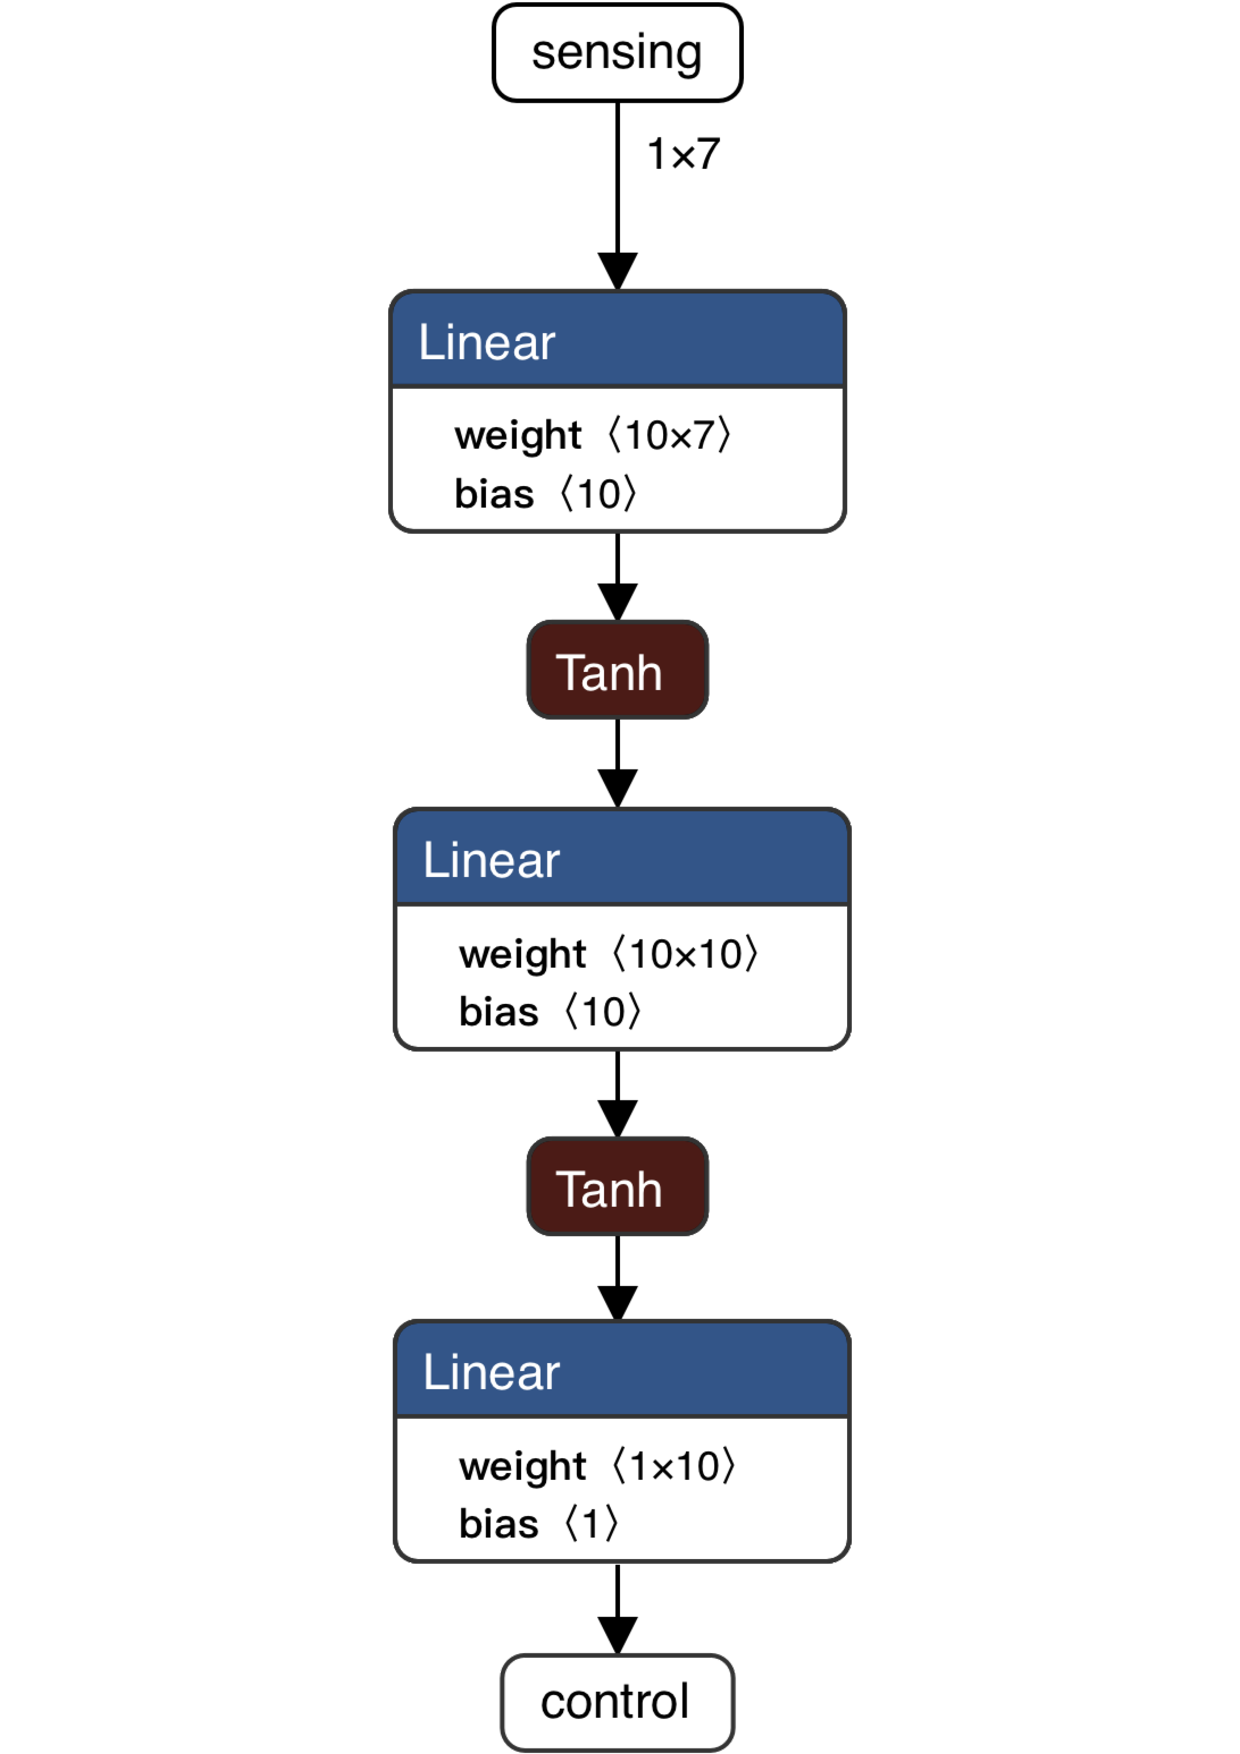
\includegraphics[width=.3\textwidth]{contents/images/task1distributed@4x}%
		\caption{Structure of a network with $7$ input sensing.}
		\label{fig:singlenet7distributed1}
	\end{subfigure}
	\hfill
	\begin{subfigure}[h]{0.495\textwidth}
		\centering
		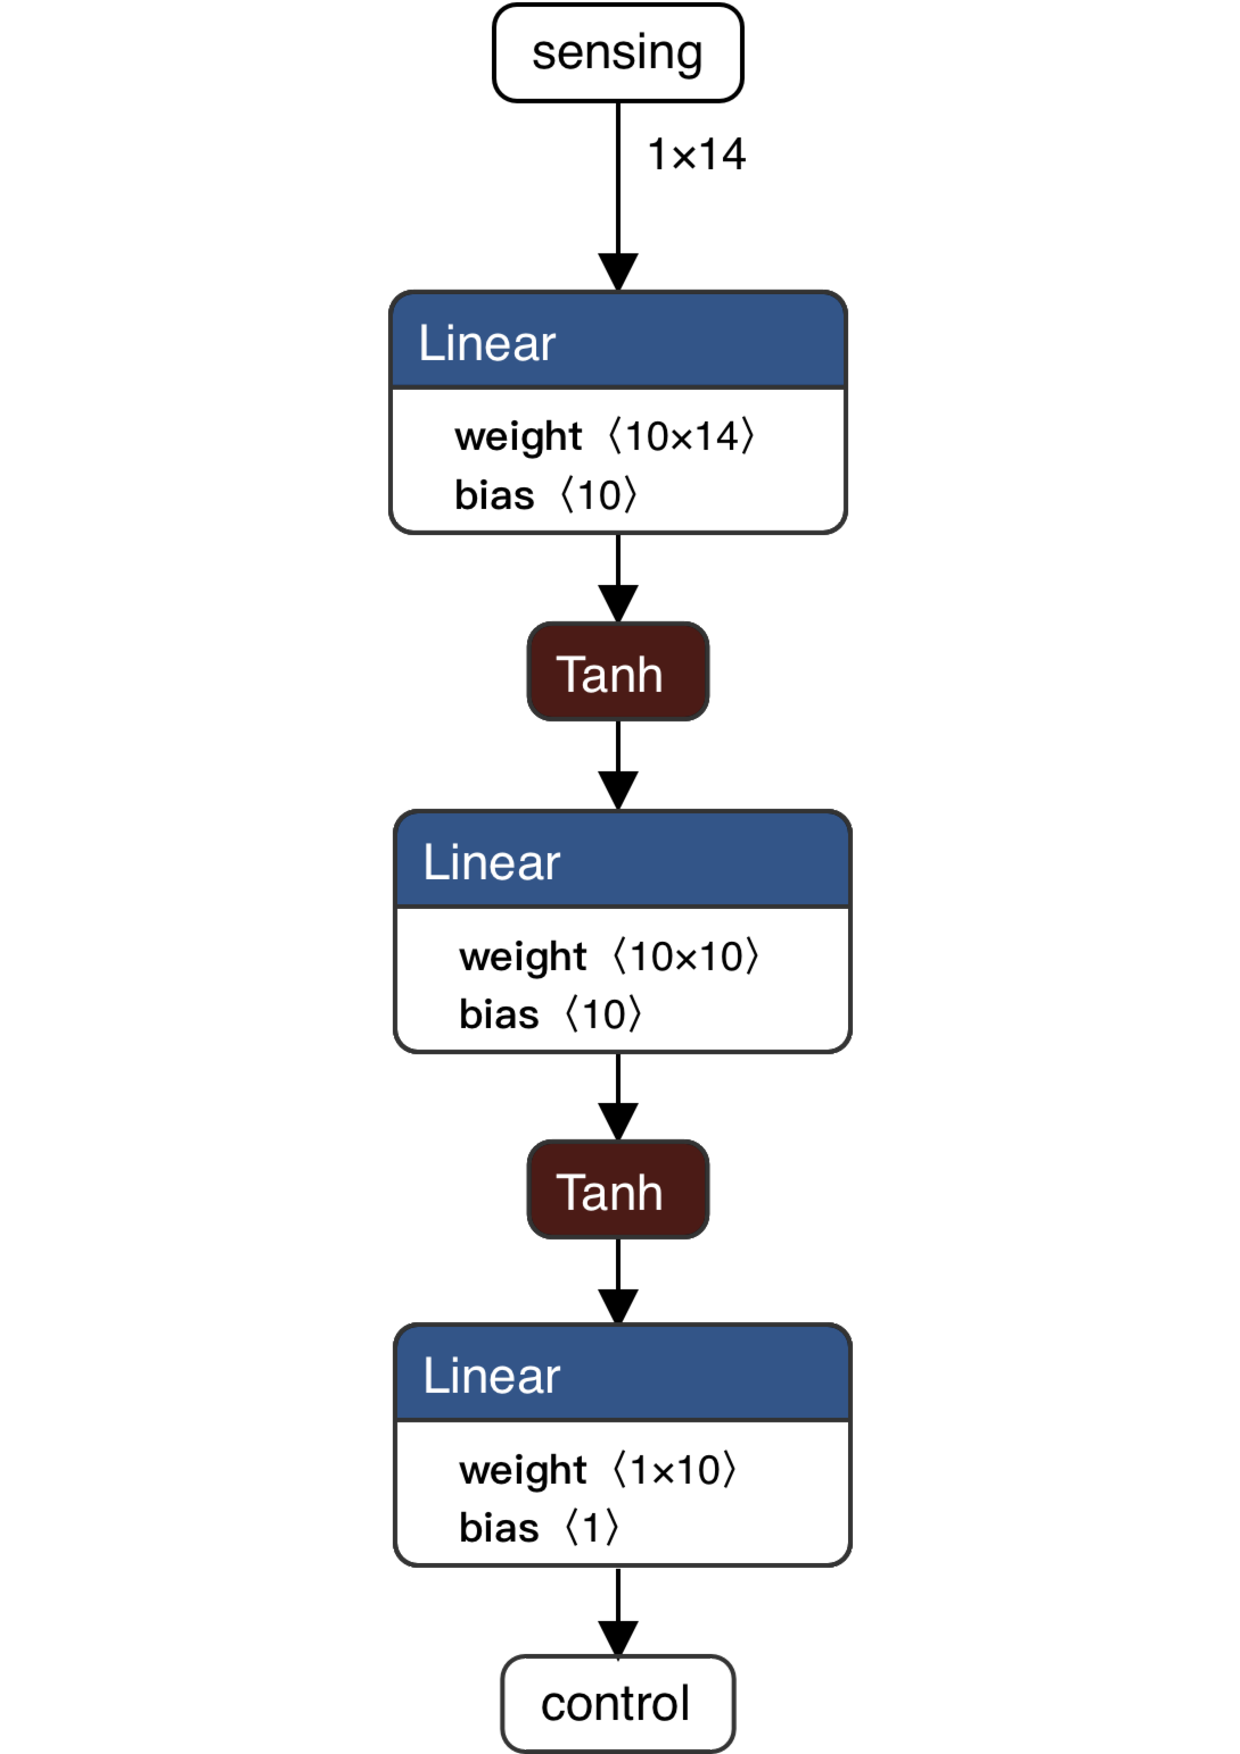
\includegraphics[width=.3\textwidth]{contents/images/task1distributed_all@4x}
		\caption{Structure of a network with $14$ input sensing.}
		\label{fig:singlenet14distributed1}
	\end{subfigure}
	\caption[Network architectures for the distributed approach.]{Visualisation of 
	the network architectures for the distributed approach.}
	\label{fig:singlenetdistributed1}
\end{figure}

To the first and second layer is applied a non-linear activation function, 
useful to make the model generalise. 
In particular, we chose the hyperbolic tangent (Tanh) 
\cite[see][]{kalman1992tanh}, a zero-centred function, shown in Figure 
\ref{fig:tanh}, whose range lies between $[-1, 1]$ and its output is given by

\begin{Equation}[H]
	\centering
	\begin{equation}
	f(x)= \frac{\sinh (x)}{\cosh (x)} = \bigg( \frac{e^x - e^{-x}}{e^x + 
		e^{-x}}\bigg)
	\end{equation}
	\caption{Hyperbolic Tangent Function (Tanh).}
	\label{eq:tanh}
\end{Equation}

This type of activation function is often used in deep learning and one of is 
advantages is that negative inputs are mapped to strongly negative values.

\begin{figure}[htb]
	\centering
	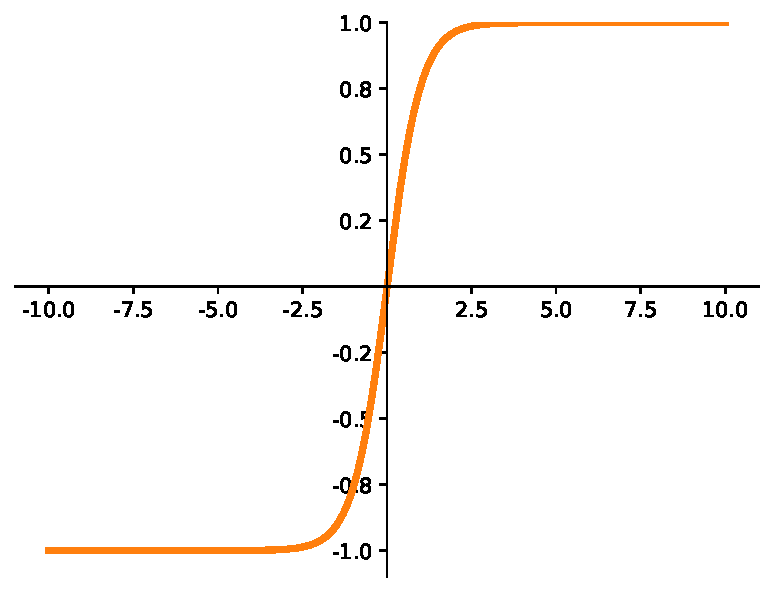
\includegraphics[width=.5\textwidth]{contents/images/tanh2}%
	\caption{Trend of the Tanh activation function.}
	\label{fig:tanh}
\end{figure}

%fixme citation
As optimiser we chose Adam, {an algorithm for first-order gradient-based 
optimisation of stochastic objective functions, based on adaptive estimates of 
lower-order moments}, \cite[see][]{kingma2014adam, 
loshchilov2017decoupled}, 
implemented in the \texttt{torch.optim} package, with a learning rate of $0.01$. 

Instead of computing the gradient descent on the entire dataset, the training set is 
split in mini-batches of size $100$ and an approximation of the gradient is 
produced, which makes the algorithm faster and at the same time, for sufficiently 
large numbers, the result is indistinguishable.

Gradient descent algorithms are susceptible to ``get stuck'' in local minima.
Mini-batches shuffle facilitate to avoid this problem by enabling the gradient to 
``bounce'' out of eventual local minimum, making it more variable by exploiting 
randomness, thereby helping convergence.

All the models are trained for $50$ epochs and evaluated using the \gls{mse} loss 
function, often used in regression problems. 
This criterion, implemented in the \texttt{torch.nn} package, measures the 
average of squared error between predictions and targets and learns to reduce it 
by penalising big errors in the model predictions.

\begin{Equation}[H]
	\centering
	\begin{equation}
	\mathtt{MSE} = \frac{\sum_{i=1}^n (y_i-\hat y_i)^2}{n}
	\end{equation}
	\caption{Mean Squared Error (\gls{mse}) loss function.}
	\label{eq:mse}
\end{Equation}
	

\subsubsection{Experiments}
\label{subsubsec:expdist}

